\documentclass[11pt,a4paper]{article}

% TIET REPORT TEMPLATE NOTE:
% Replace `article` with `tietreport` when the TIET template/class file is
% available in your LaTeX/Overleaf environment.

\usepackage[margin=0.86in]{geometry}
\usepackage[T1]{fontenc}
\usepackage{times}
\usepackage{graphicx}
\usepackage{array}
\usepackage{booktabs}
\usepackage{enumitem}
\usepackage{setspace}
\usepackage[hidelinks]{hyperref}
% Hide all hyperlink borders (including the Table of Contents links).
\hypersetup{pdfborder={0 0 0}}
\usepackage{tikz}
\usetikzlibrary{arrows.meta,positioning}
\usepackage{microtype}

\setlength{\parindent}{0pt}
\setlength{\parskip}{5pt}
\setlist[itemize]{leftmargin=18pt,itemsep=2pt,topsep=2pt}
\setlist[enumerate]{leftmargin=20pt,itemsep=2pt,topsep=2pt}
\renewcommand{\arraystretch}{1.2}

\newcommand{\statusdone}{\textbf{Completed}}
\newcommand{\statusprogress}{\textbf{In Progress}}
\newcommand{\statusplanned}{\textbf{Planned}}

\begin{document}

\begin{center}
{\Large \textbf{UCS503P -- Software Engineering Project}\\[0.35cm]}
{\LARGE \textbf{HostelFit -- Mess Calorie \& Workout Tracker}\\[0.25cm]}
{\large \textit{A Web-Based Hostel Nutrition and Fitness Tracking System}\\[0.55cm]}

\begin{tabular}{ccc}
\textbf{Aarush Sareen} & \textbf{Ishtpreet Singh Brar} & \textbf{Dhruv Singla}\\
1024160027 & 1024160022 & 1024160007
\end{tabular}

\vspace{0.45cm}
\textbf{BE Third Year, Computer Science and Engineering}\\
Thapar Institute of Engineering and Technology, Patiala\\[0.2cm]
\textbf{Progress Report -- Work in Progress}
\end{center}

\tableofcontents
\clearpage

% =============================================================
\chapter{Introduction}
% =============================================================

\section{Background and Context}
HostelFit is a web-based nutrition and fitness tracking system designed specifically for students living in hostels. The central motivation for the project is the difficulty hostel students face when trying to monitor their nutrition while having limited control over their daily food because of fixed hostel mess menus.

Unlike a generic calorie-tracking application that expects a user to search for food items individually, HostelFit is designed around the actual hostel environment. The proposed system uses pre-loaded hostel or mess menus, allows students to record the meals they consume, estimates calorie intake, records workouts and physical activity, estimates calorie expenditure, and presents an approximate daily calorie balance together with progress information.

The system has two principal roles: the Hostel Student and the Admin. Students use the application for personal nutrition and fitness tracking, while the Admin manages authorized hostel/mess menu information.

\section{Problem Statement}
Hostel students often have difficulty maintaining a structured nutrition and fitness routine because hostel mess menus are fixed, academic schedules are busy, and generic fitness applications require considerable manual effort to record hostel meals. In addition, students may not have a single platform that combines meal records, workout activity, daily calorie balance, weight history, and fitness progress.

HostelFit addresses this problem by providing a hostel-specific workflow in which the available mess menu becomes the starting point for meal tracking. The project is intended to reduce the effort of recording meals and to provide students with a unified view of nutrition, activity, and progress.

\section{Project Objectives}
The current project objectives are:
\begin{enumerate}
    \item Provide secure user registration, login, and profile management.
    \item Allow students to select fitness goals and maintain relevant profile information.
    \item Provide pre-loaded hostel or mess menu information.
    \item Allow users to log meals and estimate daily calorie intake.
    \item Allow users to record workouts and physical activities and estimate calorie expenditure.
    \item Calculate an approximate daily calorie balance using recorded nutrition and activity data.
    \item Maintain weight history and provide progress and weekly statistics.
    \item Provide an authorized Admin interface for hostel/mess menu management.
    \item Develop the system as a maintainable web application with a structured frontend, backend, and database architecture.
\end{enumerate}

\section{Current Project Status}
The project is currently \textbf{in progress}. During the initial development period, the team has completed the topic selection and presentation, established the Git repository, created and refined the system diagrams, and started the software implementation. A browser-based MVP has also been prepared to validate the main HostelFit workflow.

The complete application is not yet finished. Backend integration, persistent database operation, production-grade authentication and authorization, comprehensive testing, deployment, and final UI refinement remain part of the ongoing work.

% =============================================================
\chapter{Methodology and Design}
% =============================================================

\section{Development Methodology}
The project is being developed incrementally so that the implementation remains traceable to the requirements and system models. The current development sequence is:

\begin{center}
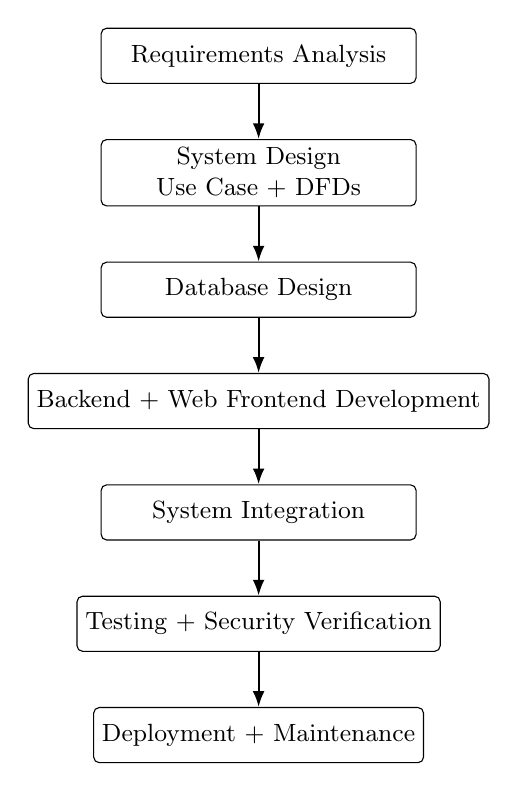
\begin{tikzpicture}[
    node distance=7mm,
    every node/.style={font=\small,align=center},
    box/.style={draw,rounded corners=2pt,minimum width=4.0cm,minimum height=7mm,inner sep=3pt},
    arrow/.style={-{Latex[length=2mm]},thick}
]
\node[box] (r) {Requirements Analysis};
\node[box,below=of r] (d) {System Design\\Use Case + DFDs};
\node[box,below=of d] (db) {Database Design};
\node[box,below=of db] (dev) {Backend + Web Frontend Development};
\node[box,below=of dev] (int) {System Integration};
\node[box,below=of int] (test) {Testing + Security Verification};
\node[box,below=of test] (dep) {Deployment + Maintenance};
\draw[arrow] (r) -- (d);
\draw[arrow] (d) -- (db);
\draw[arrow] (db) -- (dev);
\draw[arrow] (dev) -- (int);
\draw[arrow] (int) -- (test);
\draw[arrow] (test) -- (dep);
\end{tikzpicture}
\end{center}

The first three stages have already produced the main requirements and design artifacts. The implementation is currently progressing through database, backend, frontend, and integration work.

\section{System Architecture}
HostelFit is being developed as a web application with a layered architecture:

\begin{center}
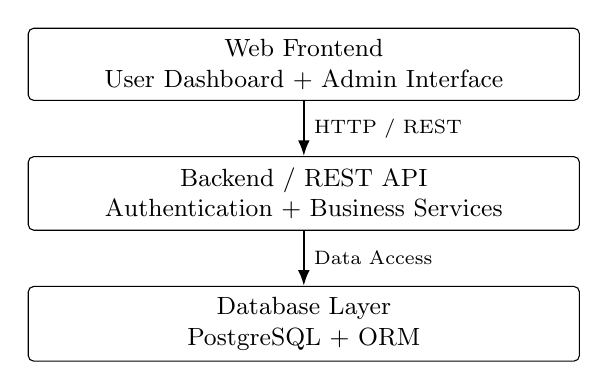
\begin{tikzpicture}[
    node distance=7mm,
    every node/.style={font=\small,align=center},
    box/.style={draw,rounded corners=2pt,minimum width=7cm,minimum height=9mm,inner sep=4pt},
    arrow/.style={-{Latex[length=2mm]},thick}
]
\node[box] (ui) {Web Frontend\\User Dashboard + Admin Interface};
\node[box,below=of ui] (api) {Backend / REST API\\Authentication + Business Services};
\node[box,below=of api] (data) {Database Layer\\PostgreSQL + ORM};
\draw[arrow] (ui) -- node[right,font=\scriptsize]{HTTP / REST} (api);
\draw[arrow] (api) -- node[right,font=\scriptsize]{Data Access} (data);
\end{tikzpicture}
\end{center}

The frontend is responsible for presenting the web interface and collecting user actions. The backend provides application services, authentication, validation, and calorie/progress calculations. The database stores persistent project information such as profiles, menus, meal records, workout records, weight records, and progress data.

\section{System Design Artifacts}
The following modelling artifacts have been prepared and refined during the design stage:
\begin{itemize}
    \item \textbf{Use Case Diagram:} Defines the interactions of the Hostel Student and Admin with HostelFit.
    \item \textbf{DFD Level 0:} Represents HostelFit as a complete system and shows its external data exchanges.
    \item \textbf{DFD Level 1:} Decomposes the system into the major profile, menu, meal, workout, calorie-balance, and progress processes.
    \item \textbf{DFD Level 2:} Decomposes meal logging and calorie-intake calculation into smaller processing steps.
    \item \textbf{Activity Diagram:} Represents the end-to-end operational flow of the student and administrative activities.
    \item \textbf{ER Diagram:} Defines the planned database entities and their relationships.
\end{itemize}

\section{Technical Stack}
The current implementation direction for the web application is:
\begin{itemize}
    \item \textbf{Frontend:} React, TypeScript, and a web-based component structure.
    \item \textbf{Backend:} Node.js with Express and TypeScript.
    \item \textbf{Database:} PostgreSQL with Prisma ORM.
    \item \textbf{Package Management:} pnpm with workspace and lockfile support.
    \item \textbf{API Style:} REST-based communication between frontend and backend.
    \item \textbf{Version Control:} Git and GitHub for collaborative development and project history.
\end{itemize}

\section{Implementation Details}
\subsection{Authentication and User Management}
The planned authentication module supports registration, login, logout, password hashing, authenticated sessions/tokens, and protected user resources. Server-side validation and authorization are required so that one student cannot access another student's personal records. This module is still under development.

\subsection{Hostel and Mess Menu Module}
The menu module provides pre-loaded menu information for the selected hostel or mess. The Admin role is intended to manage authorized menu information. The menu is then used as the data source for the student's meal-logging workflow.

\subsection{Meal and Calorie Module}
The meal module allows a student to select and log consumed meals. The system uses the associated menu and nutrition information to produce an estimated calorie intake. The design isolates the calculation logic so that formulas and nutrition data can be updated without restructuring the complete application.

\subsection{Workout and Calorie Expenditure Module}
Students can record physical activities and workout duration. The system uses the activity record to calculate an estimated expenditure value. These values are explicitly treated as estimates and not as medical measurements.

\subsection{Daily Balance and Progress Module}
The dashboard combines logged food and activity information to display an approximate daily calorie balance. Weight records are maintained over time so that the system can later provide weekly statistics, historical information, and progress visualizations.

% =============================================================
\chapter{Results and Evaluation}
% =============================================================

\section{Work Completed So Far}
The project has progressed through the following milestones:

\begin{table}[h]
\centering
\begin{tabular}{p{0.23\textwidth}p{0.16\textwidth}p{0.48\textwidth}}
\toprule
\textbf{Area} & \textbf{Status} & \textbf{Current Result} \\
\midrule
Topic and presentation & \statusdone & HostelFit topic, problem statement, objectives, motivation, and proposed solution established. \\
Git repository & \statusdone & Collaborative repository and project organization established. \\
System modelling & \statusdone & Use Case, DFD Levels 0--2, Activity, and ER design work prepared. \\
Web MVP & \statusprogress & Initial browser-based MVP demonstrates the core user workflow and interface direction. \\
Backend & \statusprogress & Backend structure and API/data requirements are being implemented. \\
Database & \statusprogress & Data model and persistence design are being refined. \\
Full integration & \statusplanned & Frontend, backend, and database integration remains to be completed. \\
Testing and deployment & \statusplanned & Comprehensive testing, security verification, and production deployment remain pending. \\
\bottomrule
\end{tabular}
\caption{Current Project Progress}
\label{tab:progress}
\end{table}

\section{Testing Methodology}
Testing is planned in layers so that individual functions are verified before complete system integration. The intended approach is:
\begin{itemize}
    \item \textbf{Unit Testing:} Test calculation functions, validation functions, and individual services.
    \item \textbf{API Testing:} Verify authentication, profile, menu, meal, workout, weight, and progress endpoints.
    \item \textbf{Integration Testing:} Verify communication between the web frontend, backend services, and database.
    \item \textbf{UI Testing:} Verify navigation, forms, dashboard behaviour, meal logging, workout logging, and progress views.
    \item \textbf{Security Testing:} Verify input validation, authentication, authorization, password handling, and protection of user-specific data.
\end{itemize}

Because the application is still under development, comprehensive final test results are not yet available.

\section{Performance Metrics}
No final performance measurements are being reported at this stage. Response time, error rate, database query performance, and other quantitative metrics will be measured after the integrated system is stable enough for meaningful testing. Reporting preliminary values without completed testing would not accurately represent the project status.

\section{Current Challenges}
The main development challenges identified so far are:
\begin{itemize}
    \item Translating the detailed system diagrams into modular software components while preserving consistency with the approved workflow.
    \item Refining the project from the original mobile-application concept into the current web-application implementation without changing the underlying functional requirements.
    \item Designing user-specific data access so authentication and authorization remain separate from ordinary application functionality.
    \item Coordinating frontend, backend, and database work so that all modules use compatible data structures and interfaces.
\end{itemize}

\section{Current Analysis}
At the current stage, the project has moved from requirements and design into implementation. The main concept has been validated through the prepared MVP workflow, while the production-oriented backend, persistent database, security controls, and automated testing are still being developed. Consequently, the present report evaluates progress and implementation readiness rather than claiming final system performance.

% =============================================================
\chapter{Conclusion}
% =============================================================

\section{Summary of Work}
HostelFit is a web-based hostel nutrition and fitness tracking system designed around fixed mess menus and the practical constraints faced by hostel students. The team has completed the initial project-selection and presentation stage, established the Git repository, prepared the main system design diagrams, and started implementation.

The design stage currently includes the Use Case Diagram, DFD Levels 0--2, Activity Diagram, and ER Diagram. The implementation direction has also been refined into a layered web architecture consisting of a web frontend, backend services, and a persistent database.

\section{Key Findings}
\begin{itemize}
    \item A hostel-specific workflow can be represented clearly through a combination of UML and DFD models.
    \item The pre-loaded mess-menu concept provides a direct link between the hostel environment and the meal-tracking workflow.
    \item Separating frontend, backend, calculation logic, and data storage provides a clearer path toward maintainable implementation.
    \item The project is sufficiently defined to continue development, but final functional and performance conclusions should be deferred until integration and testing are complete.
\end{itemize}

\section{Future Work and Remaining Implementation}
The remaining work is focused on completing the actual software system rather than expanding the scope unnecessarily:
\begin{enumerate}
    \item Complete the database schema, migrations, and controlled seed data.
    \item Complete secure authentication and authorization.
    \item Complete hostel/mess menu management and Admin functionality.
    \item Complete meal logging, calorie-intake estimation, and workout/expenditure modules.
    \item Integrate the daily calorie-balance and progress modules with persistent data.
    \item Complete the web dashboard and progress visualizations.
    \item Perform unit, API, integration, UI, and security testing.
    \item Deploy the integrated web application and prepare final documentation.
\end{enumerate}

\section{Final Remarks}
The project is currently in the implementation stage. The work completed so far has established a clear problem definition, a consistent set of system models, a development workflow, and an initial working MVP direction. The remaining stages will focus on turning these approved designs into a secure, integrated, tested, and deployable HostelFit web application.

\end{document}
